

%%%%%%%%%%%%%%%%%%%%%%%%%%%%%%%%%%
% Cells
%%%%%%%%%%%%%%%%%%%%%%%%%%%%%%%%%%
\section{Cells}
\par The cell is the basic unit of life. At the fundamental level, a cell must have an outer membrane that acts as a gatekeeper between the surrounding environment and the interior constituents. The actual contents of the cell interior vary widely between between the classes of prokaryotes (single-celled organisms) and eukaryotes (cells of multi-celled organisms), and even between different instances of the classes and different states of those instances. For example, mature red blood cells do not contain a nuclei or any genetic material, but skeletal muscle fiber consist multiple nuclei. However, all these variations can be generalized to useful cell models, such as the model for human cells in figure \ref{fig:human_cell_model}.   
\begin{figure}[ht]
 \centering
 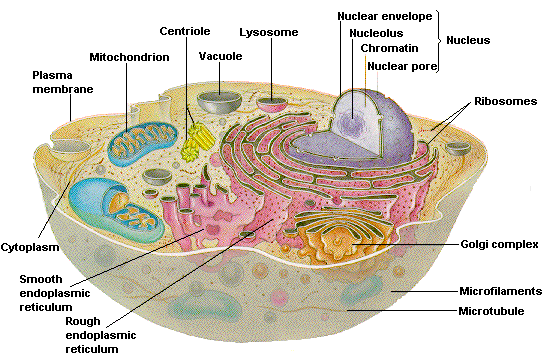
\includegraphics[width=0.7\textwidth]{images/humanCellOverview.png}
 \caption[Diagram of human cell structure.]{Diagram of human cell structure. \cite{daniel_d_chiras_human_2005} }
 \label{fig:human_cell_model}
 \end{figure}
 
 
 \par Generally, a cell carries genetic information in the nucleus inside the cell membrance and cytoplasm. Cytoplasm is all cell material inside of the cell membrane except the nuclei. The cytoplasm consists of non-nuclei organelles and cytosol.  Cytosol refers to the cellular solution between the cell organelles and the membrane, wich contains salts, nucleic acids and cytoskeleton filaments. Organnelles are membrane bound structures inside the cell that perform a special function. Organelles include nuclei, mitochondria, the Golgi apparatus, lysosomes, and vacuoles.  
 
 \par All of these 
 
 %%%%%%%%%%%%%%%%%%%%%%%%%%%%%
 % The Cell Membrane
 %%%%%%%%%%%%%%%%%%%%%%%%%%%%%
 \subsection{The Cell Membrane}
 
 
 %%%%%%%%%%%%%%%%%%%%%%%%%%%%%%%%%%%%%%%%%
 % Electrical Model of the Cell
 %%%%%%%%%%%%%%%%%%%%%%%%%%%%%%%%%%%%%%%%%
 \subsection{Electrical Model of the Cell}
 
 
 %%%%%%%%%%%%%%%%%%%%%%%%%%%%%%%%
 % Dielectric Spectroscopy
 %%%%%%%%%%%%%%%%%%%%%%%%%%%%%%%%
 \section{Dielectric Spectroscopy}

 % Read into articles and provide more details
 
 \par The dielectric properties of cells have been investigated since 1910 when H\"{o}ber showed the existence of the cell membrane by measuring the conductivity of erythrocytes (red blood cells) at high and low frequencies \cite{hober_r_methode_1910}. The field of study further developed with Fricke's application of Maxwell's equations to measure the capacitance and thickness of the cell membrane in 1924-1925 \cite{james_clerk_maxwell_treatise_1892, fricke_h_mathematical_1924, fricke_h_electric_1924, fricke_h_electric_1931}. 
 
 \par Then in 1998, Cole used Maxwell's mixture equation to derive the complex impedance of a single shelled cell model and developed equations to describe the Cole-Cole plot \cite{cole_electric_1928}. And with Curtis, Cole made the first single cell measurements on a Nitella cell \cite{curtis_transverse_1937}. A Nitella cell is a large bacteria cell that ranges in length from 20 $\mu$m to 60 mm. 
 
 \par From 1957-1968 Schwan used broadband electric impedance spectroscopy to identify $\alpha$, $\beta$, and $\gamma$ dispersions of a cell \cite{schwan_h_p_electrical_1957,schwan_h_p_electrical_1963,schwan_electrical_1994}. Where a dielectric dispersion is a frequency dependent relationship between an applied electric field and the permittivity of a material. The permittivity is the resistance to forming an electric field over a medium, and can be defined as
 \begin{equation}
     \textbf{D} = \boldsymbol{\epsilon} \textbf{E} = \epsilon_0 \textbf{E} + \textbf{P}
     \label{eqn:dielectric_displacement}
 \end{equation}
 
 % Include a discussion of the polarization tensor?
 \noindent where $\boldsymbol{\epsilon}$ is the second order permittivity tensor, $\epsilon_0$ is the permittivity of the vacuum, $\textbf{E}$ is the first order electric field tensor, $\textbf{P}$ is first order polarization density tensor which represent the density of permanent or induced electric dipole moments, and $\textbf{D}$ is the first order electric displacement tensor and represents how the electric field affects the organization or movement of charges in a medium. For a linear, homogeneous, isotropic material with instantaneous charge response, equation \ref{eqn:dielectric_displacement} can be simplified to
 \begin{equation}
    \textbf{D} = \epsilon \textbf{E}
 \end{equation}
 
 \noindent where $\epsilon$ is the zeroth permittivity tensor. 
 
 \par Examples of charge reorganization include electron cloud displacement, charge ion movement, or reorientation of molecules with dipoles. $\alpha$, $\beta$, and $\gamma$ dispersions refers to the ranges of alternating current frequencies where the permittivity decreases significantly in cells (i.e. dielectric relaxation). Figure \ref{fig:schwan_dispersions} depicts an approximate permittivity spectrum of a cell.
 
 \begin{figure}[ht]
 \centering
 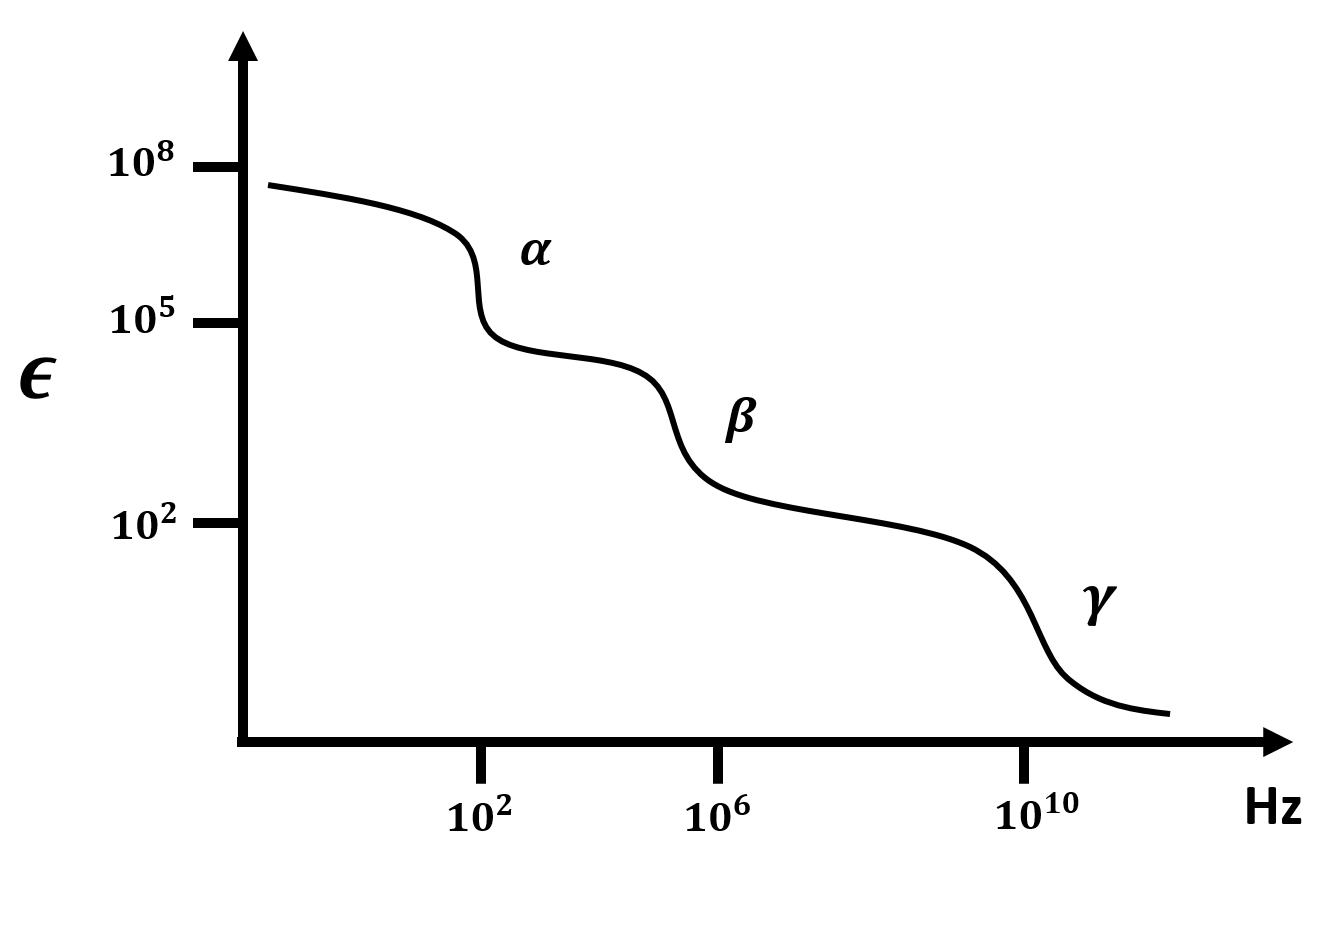
\includegraphics[width=0.7\textwidth]{images/schwanDispersions.png}
 \caption[General cell permittivity spectrum]{General cell permittivity spectrum with labeled $\alpha$, $\beta$ and $\gamma$ dispersions.}
 \label{fig:schwan_dispersions}
 \end{figure}
 
 \par $\beta$ dispersion occurs up to 10 Mhz and is caused by the relaxation of the cell membrane. For lower frequencies, the membrane has enough time to charge and provide resistance to the electric field, but at frequencies greater than about 10 Mhz, the membrane does not have sufficient time to fully charge and provides little resistance to the electric field. $\gamma$ dispersion is related to the relaxation of water molecules. Instead of a charging membrane, $\gamma$ dispersion is due to the dipole rotation of the of water molecules and the biomolecules that water is bound to. The source of $\alpha$ dispersion is undetermined, but current theories include the surface reactance of the electric double layer near the charged cell, the impedance of the sarcoplasmic recticulum (for muscle fibers), or the frequency dependent conductance of ionic membrane channels as predicted by the Hodgkin-Huxley equations \cite{schwan_electrical_1994}.
 
 
 \par These developments laid the foundations for the following techniques for measuring the dielectric properties of single cells. 
 
 %%%%%%%%%%%%%%%%%%%%%%%%%%%%%%%%
 % Dielectrophoresis
 %%%%%%%%%%%%%%%%%%%%%%%%%%%%%%%%
 \subsection{Dielectrophoresis}
 \par The dielectrophoretic force (DEP) is the force generated on a particle suspended in a solution by the interaction of an applied nonuniform electric field and an induced dipole moment developed through Maxwell-Wagner polarization (a build up of charges at dielectric boundaries). Peter Debye and Herbert A. Pohl were among the first to develop dielectrophoresis and demnostrated how particles could be moved with nonuniform electric fields \cite{muller_potential_2003}. With an applied ac electric field, the average DEP force on a spherical particle is expressed as \cite{morgan_single_2007, green_dielectrophoresis_1999}
 
 \begin{equation}
     \big< F_{DEP} \big> = \pi \epsilon_m R^3 \text{Re}[\tilde{f}_{CM}] \nabla |\textbf{E}|^2 
     \label{eqn:dep_force}
 \end{equation}
 
 \noindent with
 
 \begin{equation}
     \tilde{f}_{CM} = \frac{\tilde{\epsilon}_p - \tilde{\epsilon}_m}{\tilde{\epsilon}_p + 2\tilde{\epsilon}_m} 
     \label{eqn:fcm_background}
 \end{equation}
 
 \noindent where $\epsilon_m$ is the permittivity of the medium, $R$ is the radius of the particle, $\tilde{f}_{CM}$ is the Clausius-Mossotti factor for spherical particles,  $\tilde{\epsilon}_p$ is the complex permittivity of the particle, $\tilde{\epsilon}_m$ is the complex permittivity of the medium, and $\textbf{E}$ is the electric field. For most cases, the complex permittivity can be expressed as 
 
 \begin{equation}
     \tilde{\epsilon} = \epsilon - j\frac{\sigma}{\omega}
 \end{equation}
 
\noindent where $\epsilon$ is the permittivity, $j = \sqrt{-1}$, $\sigma$ is the conductivity, and $\omega$ is the angular frequency. 

\par From equation \ref{eqn:dep_force} and \ref{eqn:fcm_background}, it can be noted that, given an electric field, the magnitude of the dielectrophoretic force depends on the size of the particle and the polarizability of the particle with respect to the medium (i.e Re$\big[\tilde{f}_{CM}\big]$), and the sign of the force only relates to the polarizability of the particle and medium (figure \ref{fig:freq_crossover}). It should be noted that, based on equation \ref{eqn:fcm_background}, the real part of Clausius-Mossotti factor will be less than or equal to 1 and greater than or equal to -0.5. However, for non-spherical shapes, such as elongated ellipses, equation \ref{eqn:fcm_background} does not satisfy the Clausius-Mossotti factor and can reach values far greater than 1.  


\begin{figure}[ht]
 \centering
 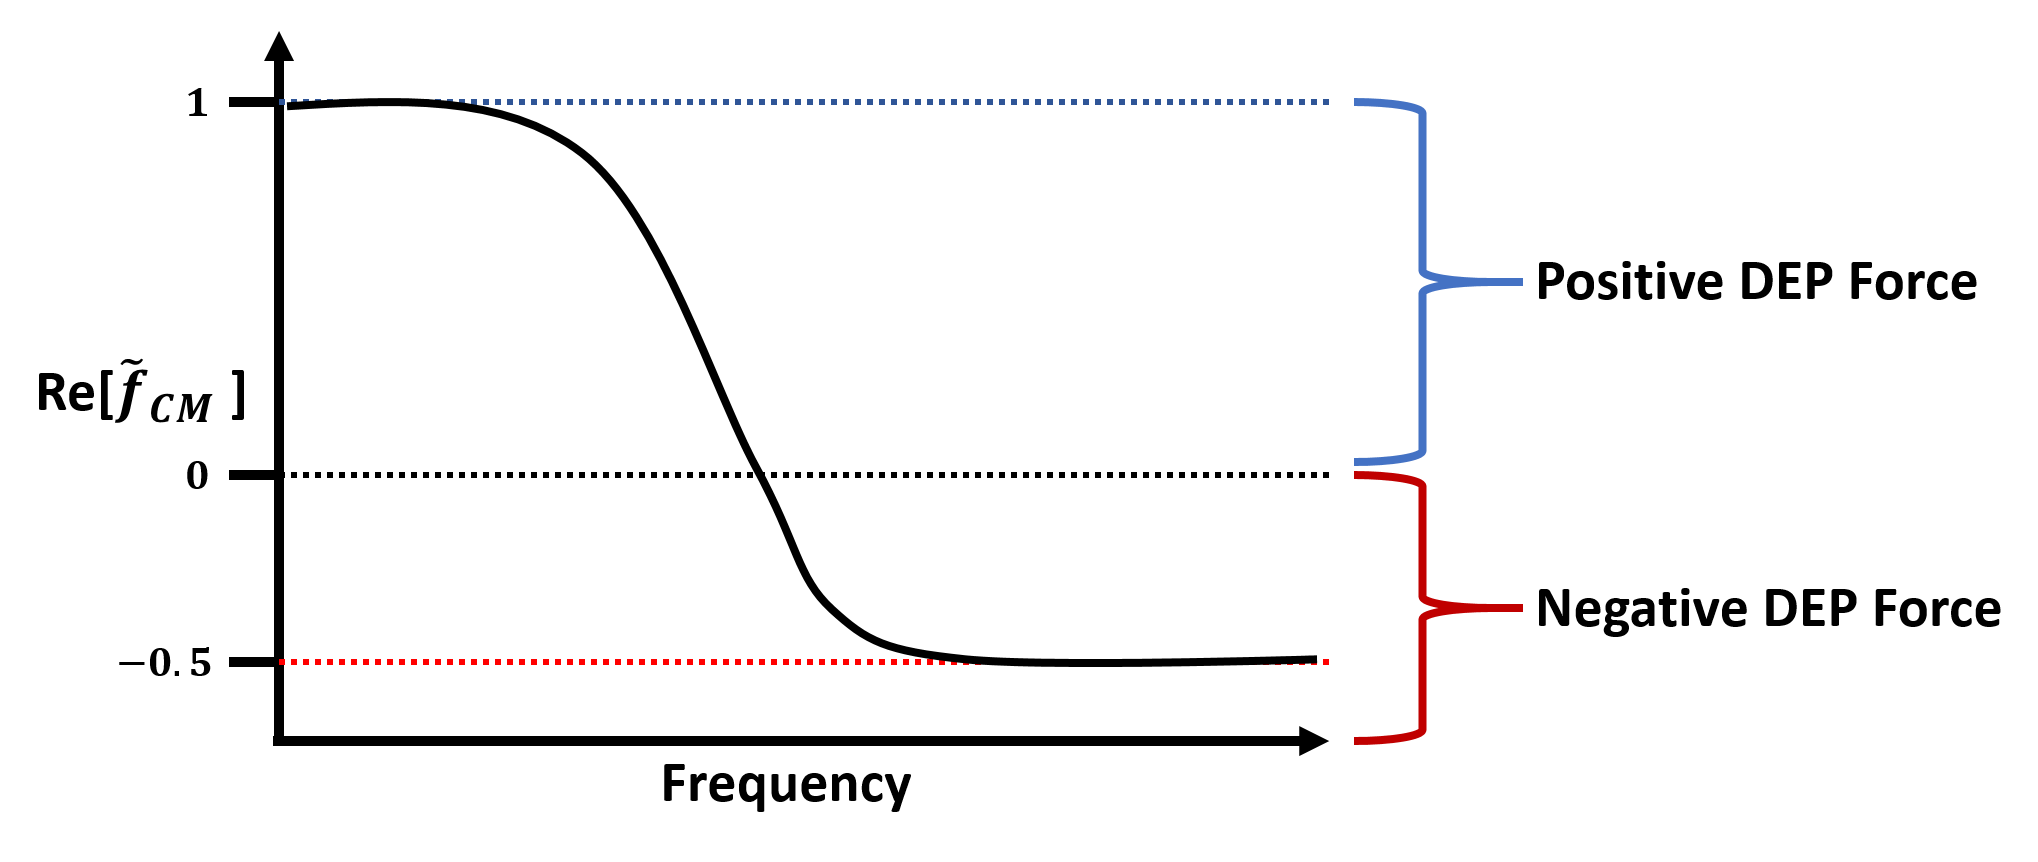
\includegraphics[width=\textwidth]{images/DEPCrossover.png}
 \caption[Frequency crossover of Clausius-Mossotti factor] {Frequency crossover of Clausius-Mossotti factor with labeled regions of positive and negative dielectriphoretic forces. From equation \ref{eqn:dep_force}, if $\tilde{\epsilon}_p$ is greater than $\tilde{\epsilon}_m$, then the DEP force is positive, if $\tilde{\epsilon}_m$ is less than $\tilde{\epsilon}_p$, then the DEP force is negative.}
 \label{fig:freq_crossover}
\end{figure}
 
 \par To extract dielectric properties of cells using dielectric forces, the DEP crossover frequency can be experimentally determined and compared to theoretical equations for the crossover frequency \cite{morgan_single_2007}. The crossover frequency occurs at the frequency when the real part of the Clausius-Mossotti factor equals zero and is where the DEP force switches from a positive to negative DEP force (or \textit{vice versa}). Experimentally, this can be determined by the observation of a stationary cell in a non-uniform electric field. Theoretically, the crossover frequency can be described as
 
 \begin{equation}
     f_{cross} = \frac{1}{2 \pi}\sqrt{\frac{(\sigma_m-\sigma_p)(\sigma_p+2\sigma_m)}{(\epsilon_p-\epsilon_m)(\epsilon_p+2\epsilon_m)}},
     \label{eqn:f_cross}
 \end{equation}
  
 \noindent where $f_{cross}$ is the crossover frequency. Equation \ref{eqn:f_cross} can be rewritten to include the Maxwell-Wagner relaxation frequency as \cite{morgan_single_2007}
 
 \begin{equation}
    f_{cross} = \frac{1}{2 \pi} \sqrt{\frac{\sigma_m - \sigma_p}{\epsilon_p - \epsilon_m}f_{MW}}
 \end{equation}
 
 \noindent with
\begin{equation}
    f_{MW} = \frac{1}{2\pi\tau_{MW}} 
\end{equation}
\begin{equation}
    \tau_{MW} = \frac{\epsilon_p + 2\epsilon_m}{\sigma_p + 2\sigma_m}
\end{equation}
 
 \noindent where $f_{MW}$ and $\tau_{MW}$ are the Maxwell-Wagner relaxation frequency and time constant respectively. The Maxwell-Wagner relaxation frequency characterizes the frequency of $\beta$ dispersion described by Schwan \cite{morgan_single_2007}.
 
 \par For a single shelled model of a cell, the crossover frequency can be expressed as
 
 \begin{equation}
     f_{cross} = \frac{\sqrt{2}}{8\pi R C_{mem}}\sqrt{(4\sigma_m - RG_{mem})^2 - 9R^2G^2_{mem}},
 \end{equation}
 
 \noindent where $C_{mem}$ is the specific capacitance of the cell membrane and $G_{mem}$ is the specific conductance of the membrane.
 
 %%%%%%%%%%%%%%%%%%%%%%%%%%%%
 % Electrorotation
 %%%%%%%%%%%%%%%%%%%%%%%%%%%%
 \subsection{Electrorotation}
 
 \par Electrorotation is the applied torque to a polarized particle in a medium of different dielectric properties by a rotating electric field. Such a field can be created with a system of four electrodes with sinusoidal signals of 90\textdegree \;phase shifts between adjacent electrodes \cite{goater_electrorotation_1999}. The phenomenon of electrorotation was first documented by by Pohl in 1978 and then developed into dependable methods by Arnold and Zimmerman in 1982 \cite{pohl_dielectrophoresis_1978-1, arnold_rotating-field-induced_1982}.
 
 \par The average torque exerted on a spherical particle can be expressed as \cite{morgan_single_2007}
 \begin{equation}
    \Tau_{\text{ROT}} = -4\pi \epsilon_m R^3 \text{Im}\big[\tilde{f}_{CM}\big]|\textbf{E}|^2
    \label{eqn:ROT_torque}
 \end{equation}
 
 \noindent where $\Tau_{\text{ROT}}$ is the torque applied to the induced dipole of the particle, $\epsilon_m$ is the permittivity of the medium, $R$ is the radius of the spherical particle, $\textbf{E}$ is the electric field, and $\text{Im}\big[\tilde{f}_{CM}\big]$ is the imaginary part of the Clausius-Mossotti factor expressed in equation \ref{eqn:fcm_background}. Similarly to the average dielectrophoretic force applied on a particle (equation \ref{eqn:dep_force}), the Clausius-Mossotti factor is the frequency dependent element and controls whether the particle rotates with or against the applied rotating electric field.
 
 \par The applied torque can be measured by the angular velocity of the particle which can be expressed as \cite{morgan_ac_2003}
 \begin{equation}
     R_{\text{ROT}} = - \frac{\epsilon_m\text{Im}\big[\tilde{f}_{CM}\big]|\textbf{E}|^2}{2\eta}K, 
 \end{equation}
 \noindent where $R_{\text{ROT}}$ is the rotation rate, $\eta$ is the dynamic viscosity, and K is the scaling factor. When the angular velocity has reached equilibrium, the applied torque will be proportional $R_{\text{ROT}}$ and related by the scaling factor K. The electrorotation torque spectrum of a cell can be used, in tandem with equation \ref{eqn:ROT_torque}, to determine the dielectric properties of the cell. 
 
 \par By combining dielectrophoretic and electrorotaion spectroscopy techniques, significant details on the dielectric properties can be obtained. Since dielectrophoretic spectroscopy obtains the real Clausius-Mossotti factor spectrum, and electrorotation obtains the imaginary Clausius-Mossotti factor, the full $\tilde{f}_{CM}$ spectrum can determined from which dielectric properties can be extracted. Seperating the real and imaginary components of the Clausius-Mossotti factor, the following expressions are obtained
 % However, a major shortcoming of the previously discussed techniques is long time for measurements. An electrorotaion assay could potentially take up to several seconds per test and, as a result, limit the number of cells tested
 
 %%%%%%%%%%%%%%%%%%%%%%%%%%%%%%%%%%%%%%%%%%%%%
 % Electrical Impedance Spectroscopy
 %%%%%%%%%%%%%%%%%%%%%%%%%%%%%%%%%%%%%%%%%%%%%
 \subsection{Electrical Impedance Spectroscopy}
 
 
 % Electrical impedance spectroscopy has historically only been used on multiple cells to obtain aggregate data, however, with the rise of microelectomechanical systems (MEMS) and microfluidics, electrical impedance spectroscopy can be applied to individualy cells.
 
 
 %%%%%%%%%%%%%%%%%%%%%%%%%%%%%%%%%%%%%%%%%%%%%%%%%%%%%%%%%
 % Microelectromechanical Systems and Microfluidics
 %%%%%%%%%%%%%%%%%%%%%%%%%%%%%%%%%%%%%%%%%%%%%%%%%%%%%%%%%
 \section[MEMs and Microfluidics]{Microelctromechanical Systems and Microfluidics}
 
 %%%%%%%%%%%%%%%%%%%
 % MEMS
 %%%%%%%%%%%%%%%%%%%
 \subsection{MEMS}
 
 
 %%%%%%%%%%%%%%%%%%%%%%%%%%
 % Microfluidics
 %%%%%%%%%%%%%%%%%%%%%%%%%%
 \subsection{Microfluidics}
 
 
 %%%%%%%%%%%%%%%%%%%%%%%%%%%%%%%%%%%%%%%%%%%%%%%%%%%%%%%%%%%%%%%%%%%
 % Previous Work on the Cal Poly Biofluidic Lab's EIS System
 %%%%%%%%%%%%%%%%%%%%%%%%%%%%%%%%%%%%%%%%%%%%%%%%%%%%%%%%%%%%%%%%%%%
 \section{Previous Work on the Cal Poly Biofluidic Lab's EIS System}
 
 % In 2009 Josh Fadriuela and Stephanie Hernandez fulfilled their thesis under Dr.Clague to create a cell impedance sensor system. Their work will be the foundation for this thesis \cite{fadriquela_design_2009-1}, \cite{hernandez_single_2009-1}.
 